\documentclass{article}
\usepackage[T1]{fontenc}
\usepackage[utf8]{inputenc}
\usepackage[francais]{babel}
\usepackage{hyperref}
\usepackage{comment}
\usepackage{graphicx}


%% first attempt (but needs modifications in case of optional parameters to \includegraphics)

\newcommand{\vcenteredinclude}[1]{\begingroup
\setbox0=\hbox{\includegraphics{#1}}%
\parbox{\wd0}{\box0}\endgroup}

%% better: (general command to vertically center horizontal material)
\newcommand*{\vcenteredhbox}[1]{\begingroup
\setbox0=\hbox{#1}\parbox{\wd0}{\box0}\endgroup}

\title{MusicBot - Propal}
\author{Alexandre Talon\and Alice Pellet-Mary\and Antoine Grospellier\and Baptiste Rozière\and Benjamin Farinier\and Diego Nava Saucedo\and François Pirot \and Pierre Macherel\and Louis Gal\and Valentin Gledel}
\date{9 octobre 2013}
\begin{document}
\maketitle
{\centering
\vcenteredhbox{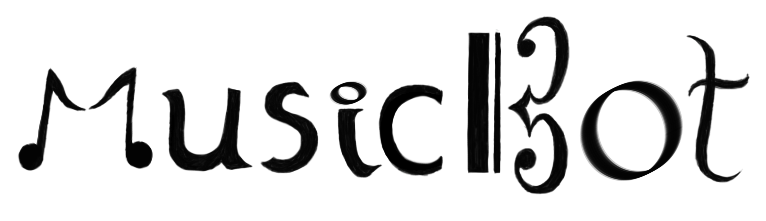
\includegraphics[width = 5cm]{logoBis}} \hfill
%\vcenteredhbox{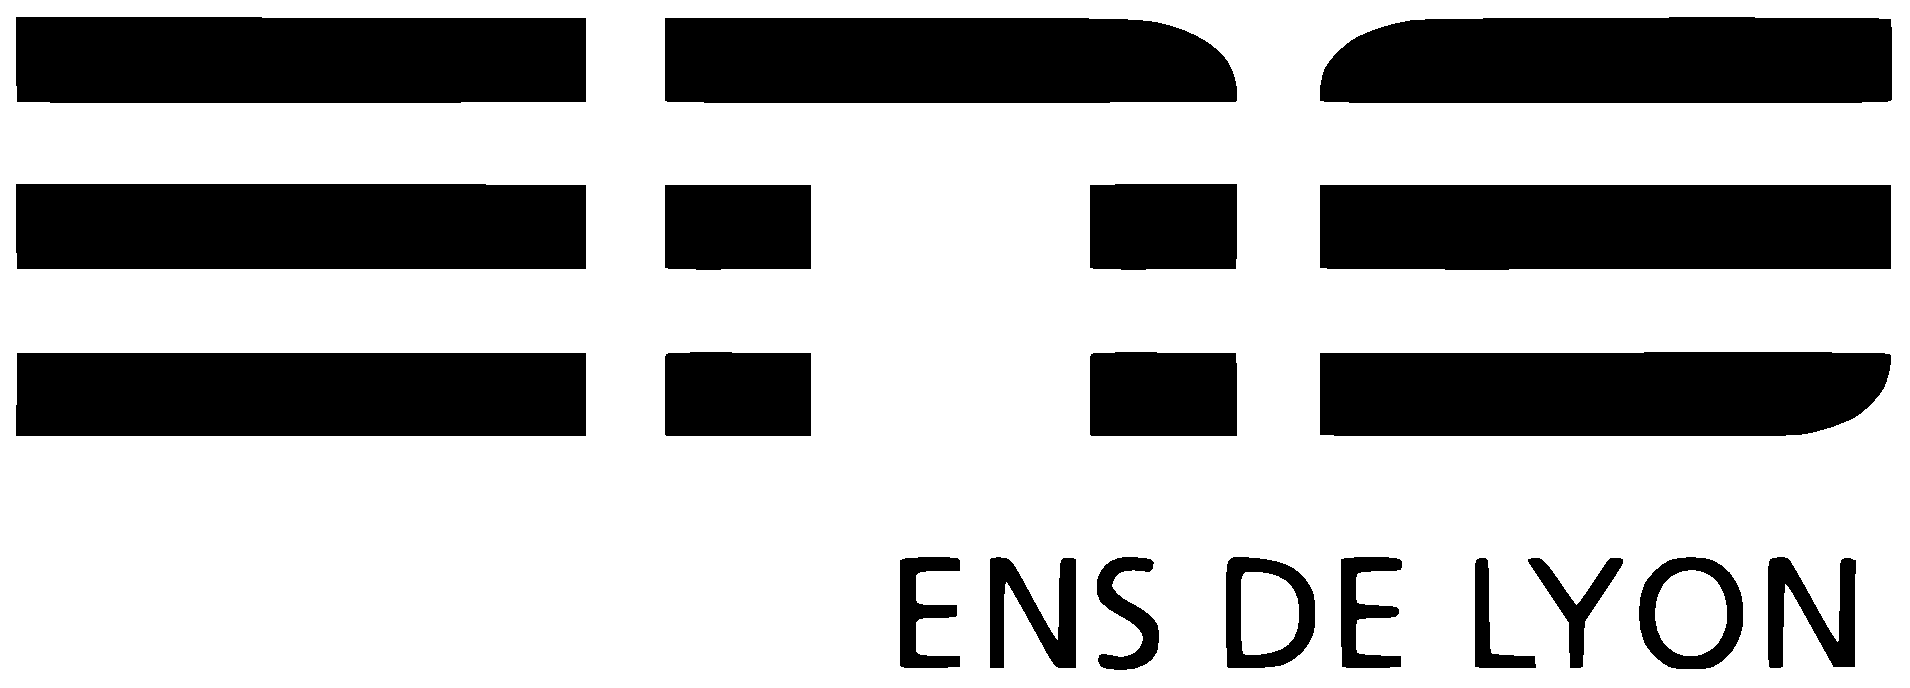
\includegraphics[width = 5cm]{ens}}
}
\section{Introduction}
\indent Pour l'instant l'utilisation des outils informatiques ou des supports numériques dans le monde de la musique est assez réduite. Si des recherches existent notamment chez les compositeurs contemporains sur les relations possibles entre les musiciens et la machine en terme de création et de dialogue, la plupart des instrumentistes utilisent des partitions papier et travaillent leurs partitions sans support électronique. \\\\
\indent Or, ces outils et supports pourraient se révéler très utiles et quelques rares initiatives existent comme le montre cet \href{http://www.lematin.ch/culture/musique/Un-orchestre-passe-des-partitions-papier-aux-tablettes/story/27663619}{article} tout en présentant les enjeux dont nous parlons. Les raisons de souhaiter la numérisation des partitions par exemple sont nombreuses. Tout d'abord, les instrumentistes portent tous les jours de lourdes partitions pour pouvoir travailler. En outre, une économie de papier serait également très souhaitable pour le développement durable. Enfin, des logiciels permettant aux musiciens d'éviter d'arrêter de jouer pour tourner les pages seraient bienvenus  et l'aide qu'apporterait un logiciel aux séances de travail individuel serait très utiles. Pour la pratique amateure, un détecteur de fausses notes pourrait les aider à améliorer leur connaissance du morceau qu'ils travaillent sans l'aide d'une tierce personne, mais ce logiciel pourrait, avec d'autres fonctionnalités intégrées, également aider des professionnels. Des applications existent déjà pour répondre à cette demande mais elles sont encore peu répandues et utilisées car souvent payantes et ne proposant que peu de partitions. \\
\\
\indent \textbf{MusicBot} se présenterait sous la forme d'un assistant musical, dont le but serait d'aider les musiciens de tous niveaux dans la phase de déchiffrage puis de travail d'un morceau. 
Il fournira donc des outils basiques permettant de faciliter la découverte et le travail de partitions, tels qu'un métronome, une gestion intelligente du défilement de la partition, ...
\\ \\ \indent En outre, il proposera une analyse critique de l'interprétation du musicien, en mettant en valeur les passages ne respectant pas exactement la partition, que ce soit au niveau de la justesse des notes, de la régularité du rythme ou de la bonne gestion des nuances. Ce sont autant de détails qu'il est difficile de gérer convenablement pour un musicien travaillant seul.
\\ \\ \indent Se voulant intuitif est à portée de tous, ce logiciel se déclinera sous la forme d'une application pour smartphone et/ou tablette, afin de pouvoir aisément suivre les musiciens lors de leurs déplacements. Son but est de regrouper des outils plus ou moins disponibles par le biais de logiciels potentiellement déjà existants, mais souvent payants  ou inaboutis. \\ \\
\indent \textbf{MusicBot} acceptera l'importation de partitions scannées, ce qui lui permettra d'avoir accès à une base de données libre sans limite, notamment par le biais de sites de partitions libres de droits tels que \href{www.imslp.org}{\textbf{IMSLP}}, ce qui la différenciera de son principal concurrent \textbf{Weezic}. L'objectif serait de créer une communauté active autour de cette application qui permettrait de l'enrichir après sa création.


\section{Membres du projet}
Les membres du projet sont Alexandre Talon, Alice Pellet-Mary, Antoine Grospellier, Baptiste Rozière, Benjamin Farinier, Diego Nava Saucedo, François Pirot, Pierre Macherel, Louis Gal et Valentin Gledel. Le chef du projet est \textbf{François}.

\section{Description}
Le projet se décompose en quatre modules principaux (work packages), en plus du work package communication. Le nom de chaque chef de work package est en gras. 

\subsection{WP0 : communication}
\noindent \textbf{Membres du WP0 : } \textbf{Baptiste}, François et Louis\\
Le but de ce work package est de fournir une documentation sur le projet au public potentiel. Il comprend notamment la création du site web du projet. Il assure également la bonne cohésion des différents work packages entre eux.

\subsection{WP1 : Numérisation de partition} 
\noindent \textbf{Membres du WP1 : } Diego, François, {\bf Pierre} et Valentin\\
Ce work package a pour objectif de parvenir à lire une partition scannée, se présentant sous la forme d'une image. Il s'agira donc de reconnaître un maximum d'informations musicales sur la partition, et de les stocker dans un format adéquat et réutilisable par la suite. Une fois ces données obtenues, il sera facile de les modifier, afin par exemple de proposer un outil de transposition de la partition dans une quelconque autre tonalité.\\
Ce module nécessite du traitement d'image afin de numériser la partition.\\
Première tâche : numériser la partition.\\
Deuxième tâche : Transposition de partition.\\
À partir d'une partition, l'objectif est d'obtenir une nouvelle partition avec le morceau transposé dans une autre tonalité.

\subsection{WP2 : Reconnaissance auditive}
\noindent \textbf{Membres: } \textbf{Alice Pellet-Mary}, Antoine GrosPellier, Baptiste Rozière, Louis Gal\\
L'objectif de ce WP est la création d'une partition de musique depuis un flux audio, stockée dans un format que le logiciel peut utiliser. Dans un premier temps, on essaye de reconnaitre une ligne monodique (un instrument seul jouant une seule note à la fois). On essaiera ensuite d'élargir la reconnaissance à des lignes musicales polyphoniques.\\
\subsubsection{Tâches}
Première tâche : Reconnaitre les notes jouées en temps réel et les envoyer au WP3.\\
Le format utilisé pour stocker les informations reconnues sera proche de celui de lilypond (pour chaque note on écrit simplement son nom, son octave et sa durée en secondes). L'objectif est pour chaque note jouée de reconnaître la note et d'obtenir sa durée.\\
Deuxième tâche : Obtenir une vraie partition à partir d'un flux audio.\\
Dans la première version, on n'a pas besoin de tous les éléments d'une partition pour pouvoir suivre le musicien. L'objectif ici serait d'obtenir plus d'informations à partir du flux audio (par exemple la fréquence exacte de la note, ou son volume) pour \^etre capable d'en ressortir une vraie partition. Ces données supplémentaires peuvent également servir à la deuxième tâche du WP3 pour analyser la justesse et l'interprétation du musicien.

\subsubsection{Choix technologiques}
On utilisera pour ce WP la bibliothèque \href{http://aubio.org/}{Aubio}, dont l'outil \texttt{aubionotes} permet d'extraire le nom des notes et leur durée en temps réel. On peut également utiliser l'outil \texttt{aubiopitch} qui renvoie la valeur précise de la fréquence à la place de l'arrondi à la note la plus proche.\\
Aubio est un outil conçu pour fonctionner seulement sur un ordinateur : il prend en charge l'enregistrement du son et sa gestion, qui n'est pas forcément la même sur une tablette ou un smartphone. De plus son code est en C avec des scripts en python, ce qui rend son portage sur android compliqué.\\
Cependant, on essayera de proposer à ceux voulant utiliser musicbot sous android un système où le smartphone servirait seulement de micro, et le travail d'aubio serait fait à distance sur un ordinateur via Internet. L'application ne pourra donc pas être utilisée sans Internet.

\subsubsection{Caractéristiques de cette portion de logicielle}
Le WP2 prend en charge l'enregistrement du musicien et renvoie un flux de notes, prises en charges par le WP3, au format (\texttt{nom\_de\_la\_note octave durée\_en\_seconde - note\_suivante}...).\\
Le WP2 se charge aussi d'obtenir, en temps réel ou après coup (si après coup, c'est lui qui est chargé d'enregistrer l'entrée pour en garder une trace), des informations supplémentaires, comme la fréquence réelle des notes, qu'il enverra également au WP3.
\subsubsection{Apports personnels}
Aubio fonctionne plutôt bien pour reconnaître les notes mais il y a quand même quelques petits problèmes : certaines notes sont renvoyées plusieurs fois alors qu'elles ne sont jouées qu'une fois (il renvoie régulièrement deux fois la même note courtes au lieu d'une seule note longue), les notes n'ont pas toujours le bon octave, certaines notes sont décalées d'un demi ton... Notre objectif est d'essayer de diminuer ces erreurs pour être le plus près possible du morceau réellement joué.


\subsection{WP3 : Synchronisation musicale}
\noindent \textbf{Membres du WP3 : } {\bf Alexandre}, Alice, Benjamin et François\\
L'objectif de ce work package est de parvenir à superposer deux flux musicaux correspondant à un même morceau. L'objectif est de réussir à mettre en correspondance une interprétation d'un morceau avec son interprétation théorique selon la lecture de la partition, et ainsi de réussir à suivre le musicien lorsqu'il joue. Cela devra se faire malgré les potentielles erreurs du musicien, qu'il s'agira par la suite de lui signaler.\\
Ce work package utilisera les partitions au format lilypond scannées par le work package 1 ainsi que le morceau enregistré et transformé par le work package 2.\\
Ce module pourra utiliser des algorithmes similaires aux algorithmes de comparaison de chaînes d'ADN pour comparer la partition et les notes entendues.
Première tâche : suivre le musicien qui joue en temps réel.\\
Deuxième tâche : Correction d'erreurs.\\
L'objectif serait de proposer au musicien une correction des erreurs qu'il a faites en jouant, soit à la fin du morceau, en lui indiquant toutes les erreurs d'un coup, soit au fur et à mesure qu'il joue.

\subsection{WP4 : GUI}
\noindent \textbf{Membres du WP4 : } Alexandre, {\bf Diego}, Louis et Pierre\\
Ce work package a pour but la création de l'interface graphique de Musicbot pour ses diverses déclinaisons : pour ordinateur, pour tablette et pour smartphone Androïd. Il s'agira aussi de trouver une manière intuitive d'afficher et faire défiler une partition sur un écran, notamment sur un petit écran comme celui des smartphones.\\

%On laisse se WP ou on pense qu'il y aura vraiment pas le temps ?
\noindent Un nouveau work package pourra \^etre crée s'il reste du temps :
\subsection{WP5: Traduction partition-tablatures (optionnel)}
Alexandre, Alice, Baptiste et \textbf{Diego}\\
L'objectif de ce paquet serait de créer des tablatures à partir de partition (pour des instruments tels que la guitare ou certains instruments à vent), ou à l'inverse de créer des partitions à partir d'une tablature (ici spécifiquement pour la guitare).


\subsection{Apports scientifiques}
Les apports scientifiques sont très variés au sein de ce projet, et répartis de façon homogène dans chacun des work packages :

\begin{itemize}
\item WP1 : Traitement de l'image dans le but d'extraire les données d'une partition depuis une numérisation. Cela se fait en respectant certaines règles théoriques venant du solfège. Les cas ambigus pourront être traités par le biais d'une interaction avec l'utilisateur.

\item WP2 : Traitement du signal et récupération des composantes principales de la mélodie entrante. Il s'agit de ne garder que l'information pure, en mettant de côté le bruit des données, ainsi que les harmoniques.

\item WP3 : Synchronisation de deux flux de données, en direct. Il faudra optimiser la superposition de deux flux similaires, au fur et à mesure de la réception du second flux.

\item WP4 : Création d'une interface graphique adaptée à chacun des supports de l'application. 
\end{itemize}

\section{Retombées}
\subsection{Objectif principal}
À terme, MusicBot aura pour ambition de se retrouver sous diverses plate-formes, allant du smartphone à l'ordinateur, et de proposer sous chacune de ses déclinaisons un assistant au travail musical complet et adapté à son support. MusicBot a une volonté d'aider le musicien à rendre son travail efficace, d'une part en lui fournissant des outils rendant la phase de déchiffrage plus confortable, et d'autre part en cernant les parties du morceau dont la réalisation est imparfaite et nécessite un travail plus approfondi et précis.

Il se veut totalement libre afin de pouvoir profiter d'une communauté prête à le faire évoluer, et de compter un nombre d'utilisateurs conséquent.

\subsection{Public visé}
Sont visés par cet assistant tous les étudiants musiciens qui n'auraient pas encore acquis une autonomie complète dans leur travail. Cela concerne notamment tous les élèves en conservatoire, qu'ils soient débutant ou bien atteignant un niveau confirmé. Chacun pourra y trouver des outils qui sauront se démontrer d'une grande aide. Cependant, MusicBot n'a pas la prétention de pouvoir remplacer un professeur !

L'utilisation de MusicBot se limite au travail d'un seul instrument à la fois. L'application n'est donc pas adaptée à une utilisation au sein d'un orchestre, ou même d'un petit ensemble d'instrumentistes. Elle intervient lors du travail individuel de chacun des musiciens.

Le portage de l'application sur le plus de plate-formes possible permettra d'élargir tout autant l'ensemble de ses potentiels utilisateurs.

\section{Concurrents}
Le principal concurrent de MusicBot serait l'application pour Ipad \href{http://weezic.com/fr/}{Weezic}, qui propose un outil d'accompagnement automatique des musiciens.
MusicBot s'en différencie en se penchant sur l'analyse des erreurs d'interprétation du musicien et en l'aidant dans son travail. De plus, nous ne sommes limités ni par le support (exclusivement Ipad pour Weezic), ni par la base de données (seules des partitions pré-formatées sont utilisables par Weezic). En plus de cela, notre contenu est entièrement gratuit, contrairement à Weezic dont les partitions pré-formatées sont payantes.


\section{Calendrier des work packages}

\begin{itemize}
\item {\bf Numérisation de partition} : 2 ou 3 mois à partir du début
\item {\bf Reconnaissance auditive} : 2 ou 3 mois à partir du début
\item {\bf Synchronisation musicale} : 1 ou 2 mois à partir du début
\item {\bf GUI} : Tout au long de l'évolution des autres WP
\item {\bf Tablature} : environ 1 mois à partir de la fin des work packages principaux
\end{itemize}
\begin{figure}
\centerline{
%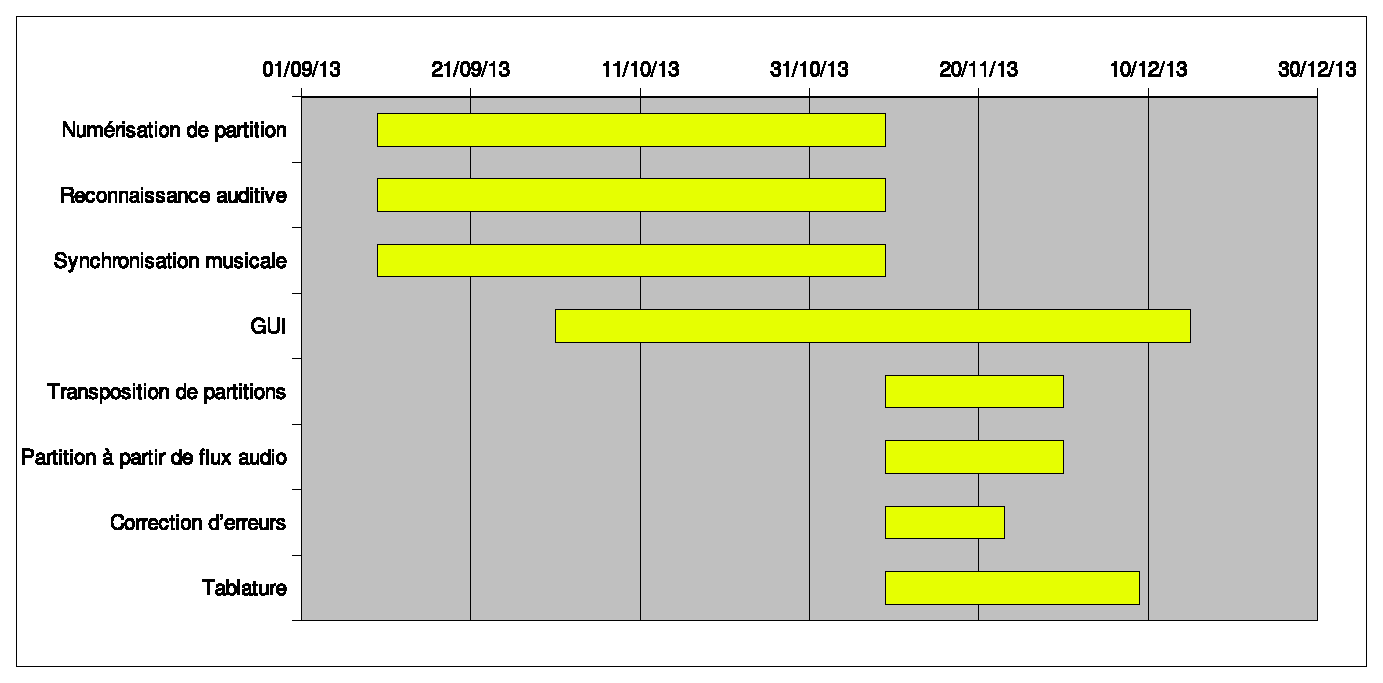
\includegraphics[scale=0.8]{grantt}
}
\caption{Diagramme prévisionnel de réalisation des work packages}
\end{figure}
\begin{figure}
\centerline{
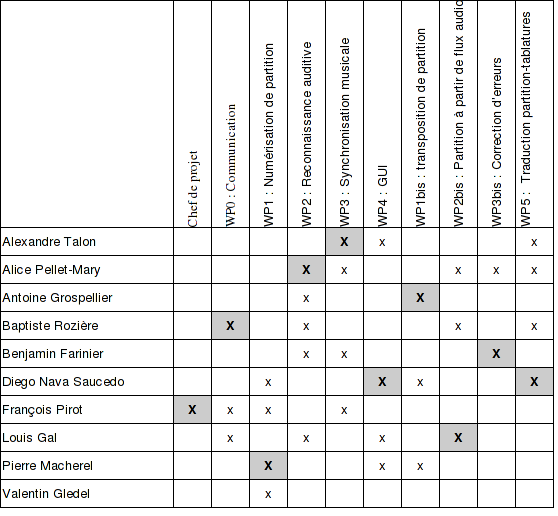
\includegraphics[scale=0.8]{aff}
}
\caption{Récapitulatif des différentes affectations. Une case grisée indique que la personne est chef du work package.}
\end{figure}



\end{document}
